\documentclass[conference,compsoc,final,a4paper]{IEEEtran}
\usepackage[utf8]{inputenx}
\usepackage{float} % for Table float parameter H

%% Bitte legen Sie hier den Titel und den Autor der Arbeit fest
\newcommand{\autoren}[0]{Karhan, Marvin}
\newcommand{\dokumententitel}[0]{Welchen Einfluss haben Dark Patterns auf Nutzer?}

% Hie muss normalerweise nichts angepasst werden
\usepackage[pdftex]{graphicx}
\graphicspath{{img/}}
\DeclareGraphicsExtensions{.pdf,.jpeg,.jpg,.png}
\usepackage[cmex10]{amsmath}
\usepackage{algorithmic}
\usepackage{array}
\usepackage{dblfloatfix}
\usepackage{url}
\usepackage[autostyle=true,german=quotes]{csquotes}
\usepackage[backend=biber,
            sorting=none,   % Keine Sortierung
            doi=true,       % DOI anzeigen
            isbn=false,     % ISBN nicht anzeigen
            url=true,       % URLs anzeigen
            maxnames=6,     % Ab 6 Autoren et al. verwenden
            minnames=1,     % und nur den ersten Autor angeben
            style=ieee,]{biblatex}
\usepackage{booktabs}
\usepackage{xcolor}
\usepackage{listings}             % Source Code listings
\usepackage[printonlyused]{acronym}
\usepackage{fancyvrb}
\usepackage{tocloft} % Schönere Inhaltsverzeichnisse

% Farben definieren
\definecolor{linkblue}{RGB}{0, 0, 100}
\definecolor{linkblack}{RGB}{0, 0, 0}
\definecolor{darkgreen}{RGB}{14, 144, 102}
\definecolor{darkblue}{RGB}{0,0,168}
\definecolor{darkred}{RGB}{128,0,0}
\definecolor{comment}{RGB}{63, 127, 95}
\definecolor{javadoccomment}{RGB}{63, 95, 191}
\definecolor{keyword}{RGB}{108, 0, 67}
\definecolor{type}{RGB}{0, 0, 0}
\definecolor{method}{RGB}{0, 0, 0}
\definecolor{variable}{RGB}{0, 0, 0}
\definecolor{literal}{RGB}{31,0, 255}
\definecolor{operator}{RGB}{0, 0, 0}

\usepackage[ngerman]{betababel}

\DefineBibliographyStrings{ngerman}{
    andothers = {{et al\adddot}},  % Immer et al. sagen, auch bei Deutsch als Sprache
}
\usepackage[
      unicode=true,
      hypertexnames=false,
      colorlinks=true,
      colorlinks=false,
      linkcolor=darkblue,
      citecolor=darkblue,
      urlcolor=darkblue,
      pdftex
   ]{hyperref}
%	 \PrerenderUnicode{ü}


% Einstellungen für Quelltexte
\lstset{
    xleftmargin=0.1cm,
    basicstyle=\scriptsize\ttfamily,
    keywordstyle=\color{keyword},
    identifierstyle=\color{variable},
    commentstyle=\color{comment},
    stringstyle=\color{literal},
    tabsize=2,
    lineskip={2pt},
    columns=flexible,
    inputencoding=utf8,
    captionpos=b,
    breakautoindent=true,
    breakindent=2em,
    breaklines=true,
    prebreak=,
    postbreak=,
    numbers=none,
    numberstyle=\tiny,
    showspaces=false,      % Keine Leerzeichensymbole
    showtabs=false,        % Keine Tabsymbole
    showstringspaces=false,% Leerzeichen in Strings
    morecomment=[s][\color{javadoccomment}]{/**}{*/},
    literate={Ö}{{\"O}}1 {Ä}{{\"A}}1 {Ü}{{\"U}}1 {ß}{{\ss}}2 {ü}{{\"u}}1 {ä}{{\"a}}1 {ö}{{\"o}}1
}

\hypersetup{
    pdftitle={\dokumententitel},
    pdfauthor={\autoren},
    pdfdisplaydoctitle=true,
    hidelinks
}

% Makros für typographisch korrekte Abkürzungen
\newcommand{\zb}[0]{z.\,B.\ }
\newcommand{\dahe}[0]{d.\,h.\ }
\newcommand{\ua}[0]{u.\,a.\ }

% Wo liegt Sourcecode?
\newcommand{\srcloc}{src/}

% Literatur einbinden
\addbibresource{literatur.bib} % Weitere Einstellungen aus einer anderen Datei lesen

\begin{document}

% Titel des Dokuments
\title{\dokumententitel}

% Namen der Autoren
\author{
  \IEEEauthorblockN{\autoren}
  \IEEEauthorblockA{
    Hochschule Mannheim\\
    Fakultät für Informatik\\
    Paul-Wittsack-Str. 10,
    68163 Mannheim
  }
}

% Titel erzeugen
\maketitle
\thispagestyle{plain}
\pagestyle{plain}

% Eigentliches Dokument beginnt hier
% ----------------------------------------------------------------------------------------------------------

% Kurze Zusammenfassung des Dokuments
\begin{abstract}
  Abstract
\end{abstract}

% Inhaltsverzeichnis erzeugen
{\small\tableofcontents}

% Abschnitte mit \section, Unterabschnitte mit \subsection und
% Unterunterabschnitte mit \subsubsection
\section{Einleitung}
Mit der immer stärker zunehmender Digitalisierung und der steigenden Anzahl an Internetnutzern \autocite{ITU2020}, wird der Einfluss von Applikationen im Internet und ihrem Design immer größer. Für ihre Nutzer ist es nicht immer klar, wenn sie ausgenutzt worden. Menschen sind besonders gut in der Erkennung von Mustern, wir nutzen die Muster verschiedener Laute, um Sprache zu verstehen und sprechen zu können. Deshalb ist es wichtig zu verstehen, welche Muster im Internet eingesetzt werden, um uns zu beeinflussen.

Viele Gelehrte befassen sich damit, Richtlinien und Vorlagen für gutes Interface Design zu verfassen. Dieses Paper beleuchtet die dunkle Seite des Interface Designs im Webumfeld. Von besonderer Bedeutung ist dabei der Einfluss von \textit{Dark Patterns} auf Nutzer. Sie sind Negativbeispiele für Interface Design und dienen nicht dem Wohle der Nutzer. Harry Brignull gilt als der Begründer des Dark Pattern Begriffs und definiert ihn als Tricks, die Nutzer dazu überzeugen, etwas zu tun, was sie ursprünglich nicht tun wollten \autocite{Brignull}. Sie nutzen psychologische Mechanismen, um die Entscheidungsfindung des Nutzers wesentlich zu beeinflussen.

% Umfang und Abgrenzung 
Diese Arbeit bietet einen Einblick in die Konzepte, die das Fundament für Dark Patterns bilden und welche rolle dabei psychologische Mechanismen einnehmen. Außerdem werden Beispiele von Dark Patterns in die von \citeauthor{Gray_2018} \autocite{Gray_2018} etablierte Taxonomie eingeordnet und bewertet. Zudem werden legislative Maßnahmen gegen Dark Patterns betrachtet und die Frage, wieso die Aufklärung von Designern und Nutzern nötig ist, beantwortet.
% Dieses Paper vermittelt einen Einblick in die Konzepte, die das Fundament für die Definition des Dark Pattern Begriffes liefern. Wie sich Dark Patterns in Applikationen manifestieren und wie Verbraucher vor Missbrauch durch Dark Patterns geschützt werden, bzw. wie können sich Nutzer davor schützen. Außerdem wird im Ausblick darauf eingegangen wie Regularien oder Nutzerverhalten den Einsatz von Dark Patterns in Zukunft beeinflussen kann.

Es wird die von \citeauthor{Gray_2018} \autocite{Gray_2018} vorgeschlagene Taxonomie verwendet, weil sie aktuell ist, anderst als die vergleichbare Taxonomie von \citeauthor{Conti2010} \autocite{Conti2010} und sicht nicht auf eine Domäne konzentriert wie die Taxonomien von \citeauthor{Lewis2014} \autocite{Lewis2014} im Bereich Mobiler Anwendungen.

% Format und Struktur (irgendwie schon im vorherigen absatz geklärt..?)

Das Ziel dieser Arbeit ist zweiseitig, einerseits soll es Designern leichter fallen, Dark Patterns in ihren Designentscheidungen zu vermeiden und anderseits sollen Nutzer leichter in der Lage sein, Dark Patterns zu erkennen, um so negative Konsequenzen zu verhindern. Ziel dieses Papers ist nicht, eine eigene Taxonomie zu erstellen oder eine vollständige Auflistung aller existierenden Dark Patterns zu bieten.


% \section{Zusätzliche Angaben}
% \subsection{Zentrale Begriffe}
% \begin{itemize}
% \item Dark Pattern
% \item Anti-Pattern
% \item evil design
% \item black hat UX
% \item dark ux
% \item Marktpsychologie
% \item CCPA (California Consumer Privacy Act)
% \item GDPR (General Data Protection Regulation)
% \item Persuasive design
% \item Deceptive design
% \item Human-centered computing
% \item Human computer interaction (HCI)
% \end{itemize}

% \subsection{Zeitplan}
% Generell ist vor jeder textuellen Abgabe entsprechend dem Umfang der Abgabe eine Rechtschreibprüfung eines Dritten angesetzt.
% \begin{table}[H]
% \begin{tabular*}{\linewidth}{ @{\extracolsep{\fill}}l  l}
%     \toprule
% \textbf{Zeitraum}                   & \textbf{Geplante Tätigkeit}       \\
%     \midrule
% 16.04 - 23.04                       & Weitere Literaturrecherche        \\
% 24.04 - 30.04                       & Kapitel 3.0 (Kapiteleinleitung), 3.1                          \\
% 01.05 - 14.05                       & Kapitel 3.2 - 3.4                          \\
% \textbf{14.05}                      & \textbf{Abgabe des Probekapitels} \\
% 15.05 - 28.05                       & Kapitel 4                           \\
% 29.05 - 11.06                       & Kapitel 5                          \\
% 12.06 - 25.06                       & Kapitel Abstract und Einleitung                          \\
% \textbf{25.06}                      & \textbf{Abgabe zum Peer-Review}   \\
% \textbf{07.07}                      & \textbf{Peer-Review (8:00 - 11:15 Uhr)} \\
% \textbf{08.07}                      & \textbf{Abgabe der Peer-Review-Bögen}   \\
% 09.07 - 16.07                       & Einarbeitung der Kritik und letzte Verbesserungen                           \\
% \textbf{16.07}                      & \textbf{Abgabe des fertigen Papers}      \\
%     \bottomrule
% \end{tabular*}
% \end{table}

% \subsection{Kontextabgrenzung}
% Dieses Paper vermittelt einen Einblick in die Konzepte, die das Fundament für die Definition des Dark Pattern Begriffes liefern. Wie sich Dark Patterns in Applikationen manifestieren und wie Verbraucher vor Missbrauch durch Dark Patterns geschützt werden, bzw. wie können sich Nutzer davor schützen. Außerdem wird im Ausblick darauf eingegangen wie Regularien oder Nutzerverhalten den Einsatz von Dark Patterns in Zukunft beeinflussen kann.

\section{Dark Patterns Grundlagen}
\label{chap:Grundlagen}
% // David Brignull als Erfinder des Begriffs 2010\\
% // wer setzt das warum ein\\
% //Neuer Einstieg\\

Traditionell nutzen Firmen Plakate und Anzeigen, um Kunden auf sich aufmerksam zu machen. Durch die Entstehung des Internets verbreitete sich das sogenannte \textit{Growth Hacking}. Mit Growth Hacking werden Marketing Aktionen bezeichnet, welche Tricks ausnutzen, um Wachstum zu steigern. Growth Hacks bewegen sich häufig an der Grenze zum illegalem  \autocite{Narayanan2020}. LinkedIn gab seinen Nutzern die Möglichkeit, automatisiert persönliche Kontakte per E-Mail zu LinkedIn einzuladen. LinkedIn versuchte an acht stellen diese Einwilligung zu erhalten und nutzte dabei zusätzlich Dark Patterns um sie zu erhalten \autocite{Schlosser2015}. Die so erhaltenen E-Mails wurden verwendet, um wiederholt E-Mails im Namen der Nutzer an deren Kontakte zu senden. Daraus resultiere eine Sammelklage, da es für die Nutzer nicht klar war, das LinkedIn die Kontakte im Namen des Nutzers mit werbe Mails spammen würde \autocite{Strange2015}. Solche Marketing Aktionen sind der Ursprung von Dark Patterns.

Dieses Kapitel ordnet Dark Patterns ein und beschreibt, wie die menschliche Psyche ausgenutzt werden kann, was \textit{Nudging} ist und anhand eines Beispiels wie \textit{Nudges} eingesetzt werden können.
\subsection{Anti-Pattern}
% // Anti-Pattern als Überbegriff von Dark Pattern und Einleitung in das Thema\\
Pattern sind der Bauplan einer Lösung zu einem wiederkehrenden Problem. Sie existieren in vielen Anwendungsbereichen \autocite[S. 1]{MacDonald2019}.

Anti-Pattern ist ein Sammelbegriff für Pattern, welche wiederkehrende Lösungen liefern, aber dabei mehr Probleme erzeugen als lösen \autocite[S. 193-195]{MacDonald2019}. Wie sich aus dem Namen bereits erschließen lässt, sind Dark Patterns eine spezifische Pattern-Art.

Unternehmen setzen Dark Pattern ein, um ihre Reichweite zu erhöhen. Das schafft Probleme aufseiten der Nutzer, da der Nutzer ausgenutzt und Profit über Nutzerfreundlichkeit gestellt wird \autocite{Chivukula_2019}, zählen Dark Patterns zu der Familie der Anti-Pattern.
\subsection{Psychologie}
\label{chap:Psychologie}
% // Warum spielt Psychologie eine rolle bei Dark Patterns?
% \\// Wie werden Nutzer von Dark Pattern beeinflusst?
% \\// Diskussion verschiedener erhobenen Statistiken zu Nutzerverhalten:\\
Dark Patterns nutzen psychologische Mechanismen aus, um Nutzer zu bewegen, etwas ungewollt oder unbewusst zu tun \autocite{Brignull}. Dafür nutzen sie oft kognitive Verzerrung, nutzen also mit speziellen Techniken die Denkweise unseres Gehirns aus \autocite{Mathur2019}.

Eine weitverbreitete Technik im Einzelhandel ist die psychologische Preisgestaltung. Das heißt, der Preis eines Produkts wird knapp unter einer runden Zahl angesetzt. Diese Technik ist schon seit mehreren Jahrzehnten im Einsatz und laut \citeauthor{Bizer_2005} (\citedate{Bizer_2005}) \autocite{Bizer_2005} ein effektives Mittel zur Verkaufssteigerung. Im Gegensatz dazu steht \citeauthor{Wieseke_2015} \autocite{Wieseke_2015} Studie aus dem Jahr \citedate{Wieseke_2015}, die sagt: Runde Preise sorgen für die höchstmögliche Verkaufswahrscheinlichkeit, da diese bequemer für den Käufer sind. Ein vergleichbarer Effekt kann bei Dark Patterns auftreten. Im ersten Schritt sorgt der Einsatz von Dark Patterns für eine höhere Nutzerbindung, jedoch im zweiten Schritt zu einer gegenläufigen Wirkung \autocite{M.Bhoot2020}.

Schon in der Zeit vor der digitalen Revolution wurden die Effekte kognitiver Verzerrung untersucht. Die Ergebnisse dieser Untersuchungen geben Aufschluss über die Manifestierung von Dark Patterns in der menschlichen Psyche.

\citeauthor{Tversky453} \autocite{Tversky453} zeigen in ihrer Untersuchung des Framing-Effekts, wie die Darstellung eines Problems das Ergebnis beeinflusst: Probanden treffen eine andere Auswahl, obwohl sich nur die Darstellung des Problems geändert hat. Konkret mussten die Probanden im ersten Problem konsekutiv eine aus zwei Möglichkeiten wählen, dabei handelte es sich um die Chance, Geld zu gewinnen oder zu verlieren. In einem anderen Problem wurden die zwei meist gewählten so wie die anderen zwei anderen Optionen zusammengefasst. Nach der Kombinierung der zwei Aussichten entschieden sich 100\% auf die vorher kaum gewählten Optionen. Diese psychologische Betrachtung lässt sich leicht auf Dark Patterns ausweiten, da Designer in einem Webumfeld weitreichende Möglichkeiten haben, um Information so zu vermitteln, dass der Nutzer nur durch ihre Darstellung zu einer anderen Entscheidung gedrängt wird.
\subsection{Nudging}
% // Vorhersehbares Beeinflussen von Nutzern um ein gewünschtes Ziel zu erreichen\\
Richard H. Thaler ist Nobelpreisträger für Wirtschaftswissenschaften. Er ist zusammen mit Cass R. Sunstein der Autor des Buchs \citetitle{Thaler2008} \autocite{Thaler2008}, der den Begriff \textit{Nudge} geprägt hat.

Er bezeichnet Personen, die Macht über den Kontext haben, indem andere Entscheidungen treffen als \textit{choice architects} \autocite[S. 3]{Thaler2008}. Im Fall von Dark Patterns sind meistens Designer diejenigen, die Thaler und Sunstein als \textit{choice architects} bezeichnen. Ihre Werkzeuge sind die psychologischen Effekte und Techniken.

\textit{To nudge} bedeutet im herkömmlichen Sinne, jemanden sachte berühren oder schubsen \autocite{MerriamWebsterNudge}. Wir werden den Begriff wie Thaler und Sunstein im übertragenen Sinne nutzen, wobei \textit{nudge} meint, jemanden mithilfe kleiner Anreize zu einem wünschenswerten Ziel zu drängen. Denn schon mit nur kleinen Anreizen kann der Nutzer zu einer anderen Entscheidung gedrängt werden \autocite{Narayanan2020}.

\begin{figure}[!ht]
  \centering
  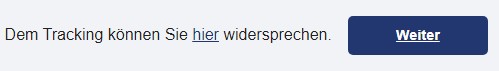
\includegraphics[width=\linewidth]{hochschule_cookie_banner}
  \caption{Eigene Aufnahme des Tracking-Banners der Hochschule Mannheim~\autocite{HSMAWebsite2021}}
  \label{fig:HSMATracking}
\end{figure}

\begin{figure}[!ht]
  \centering
  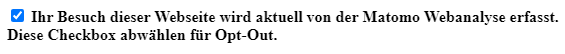
\includegraphics[width=\linewidth]{tracking_optout}
  \caption{Eigene Aufnahme der Tracking-Opt-out-Checkbox der Hochschule Mannheim~\autocite{HSMAWebsite2021}}
  \label{fig:HSMAOptOut}
\end{figure}

Um \textit{Nudging} besser zu verstehen, betrachten wir ein Dark Pattern, welches sich auf der Homepage der Hochschule Mannheim finden lässt. In \autoref{fig:HSMATracking} ist ein Ausschnitt des Tracking-Banners der Hochschule Mannheim zu sehen. Die Zustimmung zu nicht essenziellem Tracking wird hinter einem prominent dargestelltem \textit{Weiter} Button verborgen. Um eine konträre Entscheidung zu treffen, muss der Nutzer auf den weit weniger Prominenten \textit{hier} Link klicken. Dieser führt zu der Datenschutzerklärung der Hochschule in der nach der in \autoref{fig:HSMAOptOut} dargestellten Checkbox gesucht werden muss, um das Tracking zu deaktivieren. Auffällig ist, dass in dem Text das Wort \textit{tracking} nicht vorkommt. Hier wurden mehrere \textit{Nudges} genutzt, um den Nutzer dazu zu bewegen, das Tracking zu akzeptieren. Erst wird der Nutzer zum direkten Akzeptieren durch einen auffälligeren Button \textit{genudged}, danach wird der Nutzer durch das erschwerte Abwählen des Trackings in Richtung der Akzeptanz des Trackings \textit{genudged}.

Zusammenfassend lässt sich sagen, dass Dark Patterns als Zusammenschluss verschiedener Nudges verstanden werden kann.

\section{Kategorien von Dark Patterns}
% Bilder aus Kapitel 3. Nudging (HSMA) einordnen + zweites Dark Pattern (confirm shaming) direkt über
\citeauthor{Gray_2018} \autocite{Gray_2018} Ansatz nutzt \citeauthor{Brignull}'s \autocite{Brignull} Taxonomie, die primär als Resultat verschiedener Beispiele entstanden sind, und kombiniert sie, zusammen mit eigens Definierten Dark Patterns, in Kategorien. Die Kategorisierung basiert auf den Beweggründen welche Designer mit dem Einsatz der Dark Patterns haben.

\citeauthor{Gray_2018} \autocite{Gray_2018} Ansatz eignet sich gut für das Ziel dieses Papers, da durch ihre Kategorisierung der Bogen von der Intention der Designer zu den Auswirkungen auf den Nutzer geschlagen werden kann. Ohne dabei auf jedes einzelne Dark Pattern einzugehen. Denn es ist nicht wichtig, dass der Leser jedes Dark Pattern auswendig kann. Zudem können Design Elemente oft mehreren Dark Patterns und/oder Kategorien zugeordnet werden.

Jede Kategorie wird kurz erläutert und mithilfe eines repräsentativ Beispiels/Beispielen für ein Dark Pattern genauer betrachtet. Dabei wird herrausgestellt, welche Faktoren wichtig für die Erkennung des Dark Patterns sind.

Ziel dieses Abschnittes ist es, das der Leser potenzielle Dark Patterns leichter erkennt und einordnen kann, um sich dadurch besser vor ihnen schützen zu können.
\subsection{Nagging}
% Nerven bis man ja sagt (Z.B. iPhone Apple Pay-Einrichtung or No Button for No)
Nagging Dark Patterns zeichnen sich durch minimale Abweichungen der erwarteten Funktionsweise, über eine oder mehrere Interaktionen, aus \autocite{Gray_2018}.

\begin{figure}[!ht]
  \centering
  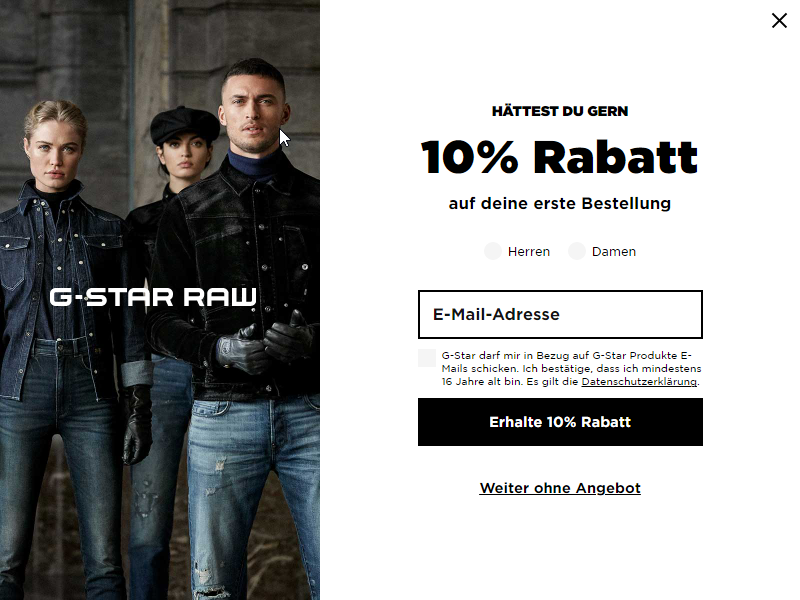
\includegraphics[width=\linewidth]{gstar_pop_up}
  \caption{Eigene Aufnahme Rabatt-Pop-ups von g-star.de~\autocite{GStar2021}}
  \label{fig:GStar2021}
\end{figure}

In \autoref{fig:GStar2021} ist Rabatt-Pop-ups von g-star.de zu sehen. Es erscheint zum erstenmal direkt nach dem Akzeptieren der Cookies und dann nach unbestimmter Zeit wieder, in leicht abgewandelter from. Ziel ist es an die E-Mail-Adresse des Nutzers zu gelangen. Dieses Dark Pattern ist wie alle Nagging Dark Pattern mit dem Zwang verbunden, dass der Nutzer damit interagieren muss \autocite{Gray_2018}, so ist es sehr leicht für nutzer sie zu erkennen.

Vorallem bei Mobilen Applikationen muss au Nagging Dark Patterns geachtet werden, dort sind sie die häufigst vertetene Dark Pattern Kategorie \autocite{DiGeronimo2020}.

\subsection{Obstruction}
\label{chap:Obstruction}
Obstruction Dark Patterns sorgen dafür, das Aktion schwerer sind als sie seien müssten, mit dem Hintergedanken den Nutzer davon abzubringen die Aktion abzuschließen \autocite{Gray_2018}.

Besitzen Sie einen Amazon-Account, wissen Sie, wie einfach es ist, einen solchen zu erstellen, es sind nur wenige Klicks nötig und der Ablauf ähnelt stark anderen Shopping-Webseiten. Will der Nutzer jedoch seinen Account löschen, ist das weit schwieriger. Die meisten Nutzer werden versuchen, unter \textit{Mein Konto} ihren Account zu löschen, aber keiner der links dort gibt dem Nutzer die Möglichkeit, seinen Account zu löschen. Um einen Amazon-Account zu löschen, ist es erforderlich, die Amazon Kundenservice Webseite aufzurufen, dort unter \textit{Hilfethemen durchsuchen}, \textit{Datenschutz} anklicken und darunter \textit{Kontaktieren Sie uns} anklicken. Danach öffnet sich eine neue Seite, in der \textit{Fragen zum Datenschutz} angeklickt werden muss. Wodurch sich eine neue Seite öffnet, auf der in einem ersten Dropdown \textit{Datenschutzauskunft} und in einem zweiten Dropdown \textit{Konto schließen und Daten löschen}, selektiert werden muss. Schließlich können, nachdem Amazon aufzählt, welche Produkte und Services ohne einen Amazon-Account nicht mehr nutzbar sind, ihren Account schließen. Alternativ kann man statt dem letzten Schritt sich per E-Mail über die Konsequenzen einer Accountschließung informieren lassen und über eine Antwort per Mail den Account schließen. Das ist ein Beispiel für \citeauthor{Brignull}'s Dark Pattern \textit{Roach Motel}, eine Situation, die einfach zugänglich ist, aber aus der es schwer ist, wieder herauszukommen \autocite{Brignull}. Wie die Untersuchung des Facebook-Account Deaktivierungsprozesses zeigt, benötigen Nutzer mit Nutzung der Googlesuchfunktion vier- bis achtmal so lange, wie es normalerweise dauern sollte, um die durch das Dark Pattern erschwerte Aktion durchzuführen \autocite{M.Bhoot2020}.

Der Zweck davon ist es, dem Nutzer möglichst schwer zu gestalten, eine ungewollte Aktion aus Sicht der Webseiten Betreibers durchzuführen. Das resultiert in mehr Mach und Profit aufseiten der Unternehmen.

Das Roach Motel Dark Pattern beruht auf keiner kognitiven Verzerrung \autocite{Mathur2019}, es hilft also nicht, aktiv auf dieses Dark Pattern zu achten, um es vermeiden zu können. Zudem gibt es auch keine anderen Faktoren, die maßgeblich zu Erkennung dieses Patterns führen, das führt dazu des es das von Nutzern am seltensten erkannte Dark Pattern ist \autocite{M.Bhoot2020}.
% von gray: pirce comparison prevention(brignull); intermediate currency
\subsection{Sneaking}
% Versteckte Kosten, sneak into basket, versteckte Subscriptions, z.B. hinter einem free trial
Sneaking Dark Patterns versuchen Informationen zu verbergen, zu verschleieren oder zu verzögern, die für den Nutzer relevant sind \autocite{Gray_2018}.

\begin{figure}[ht!]
  \centering
  \includegraphics[width=\linewidth]{airbnb_com_compare}
  \caption{Eigene Aufnahme von airbnb.com, links die Kartenansicht und rechts die Detailansicht ~\autocite{airbnb2021}}
  \label{fig:airbnb2021}
\end{figure}

In \autoref{fig:airbnb2021} werden zwei Ausschnitte der amerikanischen airbnb Webseite gezeigt, links ist die Kartenansicht von airbnb zu sehen, auf ihr kann der Nutzer alle verfügbaren objekte, die in der region buchbar sind mit ihrem Preis pro nacht sehen. Auf der rechten seite der \autoref{fig:airbnb2021} ist die Preisdetialansicht des in der Karte ausgewählten Zimmers zu sehen. In der Kartenansicht sind Zusätzliche Kosten wie die \textit{Reinigungsgebühr} und die \textit{Service-Gebühr} nicht offengelegt. Das ist ein Fall des \textit{Hidden Costs} Dark Patterns von \autocite{Brignull} \autocite{Brignull}, da hier wichtige Information für den Nutzer später als nötig preisgegeben wurden.

Die versteckten zusatz Kosten variieren von Objekt zu Objekt, sodass ein Preisvergleich verschiedener Objekte über die Kartenansicht für den Nutzer nutzlos ist. Der Nutzer müsste sich jedes Objekt in der Detailansicht anschaun und sich die Preise merken, um sie miteinander zu vergleichen. Zusätzlich werden die Versteckten Kosten unter dem Reservierungs-Button angezeigt und fallen dem Nutzer überhaupt nicht, vor der Reservierung auf.

\subsection{Interface Interference}
% Manipulation of the user interface that privileges certain actions over others.
Als Interface Interference Dark Pattern zählt jede Manipulation der Benutzeroberfläche, die bestimmte Aktionen gegeüber anderen bevorteilt und dadurch den Nutzer verwirrt oder die Sichtbarkeit wichtiger Handlungsmöglichkeiten einschränkt \autocite{Gray_2018}.

\begin{figure}[!ht]
  \centering
  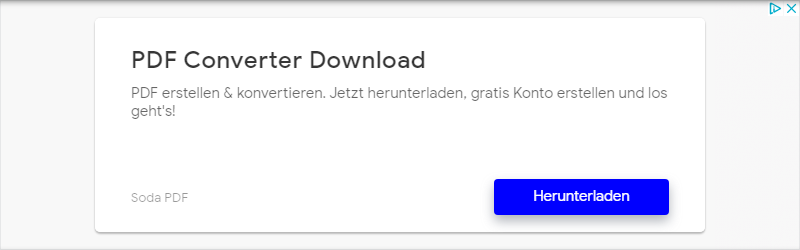
\includegraphics[width=\linewidth]{disguised_ad}
  \caption{Eigene Aufnahme einer Werbeanzeige auf chip.de von Google AdSense~\autocite{ChipAd}}
  \label{fig:ChipAd}
\end{figure}

In \autoref{fig:ChipAd} sieht man eine Werbeanzeige auf der Webseite chip.de die über Google AdSense angezeigt wird. Sie wird direkt über dem Download einer PDF-Lese Anwendung gezeigt. Das Drücken des \textit{Hernunterladen-Buttons} führt zu der Seite eines drittens. Hierbei handelt es sich um das von \citeauthor{Brignull} \autocite{Brignull} definierte Dark Pattern \textit{Disguised Ads}, Werbung die sich als Inhalt oder Navigationselement ausgibt, um häufiger angeklickt zu werden.

Die Werbung aus \autoref{fig:ChipAd} wird ganz oben auf der Webseite, vor dem tatsäch gesuchtem Download anzezeigt und nutzt den in \autoref{chap:Psychologie} beschriebenen Framing-Effekt, um dem Nutzer ein Produkt zu vermitteln, das er nicht sucht. Nutzer die schon erfahrung mit Disguised Ads gemacht haben und durch sie Frustration erfahren haben, sind besser darin sie zu erkennen \autocite{M.Bhoot2020}.

Bei Interface Interference Dark Patterns wird außerdem oft mit versteckten Informationen und vorausgewählten Standartwerten gearbeitet \autocite{Gray_2018}. Deshalb ist es für diese Kategorie von Dark Patterns wichtig, dass der Nutzer weiß, wo er nach der Information suchen muss und sortieren kann was für ihn wichtige Informationen sind. Jehäufiger der Nutzer Interface Interference Dark Patterns begegnet desto einfacher ist es sie zu erkennen und zu vermeiden \autocite{M.Bhoot2020}.

\subsection{Forced action}
% Wenn man gezwungen wird, etwas zu tun, was man nicht will und was nicht erforderlich ist, z.B. Annehmen eines Newsletters zur Anmeldung oder das Liken einer Seite, um sie zu besuchen
Forced Action Dark Patterns umfassen jede Situation, in der Benutzer eine bestimmte Aktion ausführen müssen, um auf (oder Weiterhin auf) eine bestimmte Funktionalität zugreifen zu können. Diese Aktion kann ein erforderlicher schritt oder eine Option sein, die als Großer Nutzen für den Nutzer getarnt ist \autocite{Gray_2018}.

Das in \autoref{chap:Grundlagen} erwähnte LinkedIn Dark Pattern wird von \citeauthor{Brignull} \autocite{Brignull} als \textit{Friend Spam} eingeordnet und von \citeauthor{Gray_2018} \autocite{Gray_2018} unter dem Begriff \textit{Socail Pyramid} subsummiert. Nutzer müssen hier vorallem bei Sozial-Media Anbieter aufpassen ihre Kontakte der Seite zu teilen, da das wie im Fall von LinkedIn im ersten Schritt immer als Vorteil getarnt ist, aber der Nutzer weiß nicht und hat keinte Kontrolle darüber was mit diesen Daten passiert.

\begin{figure}[!ht]
  \centering
  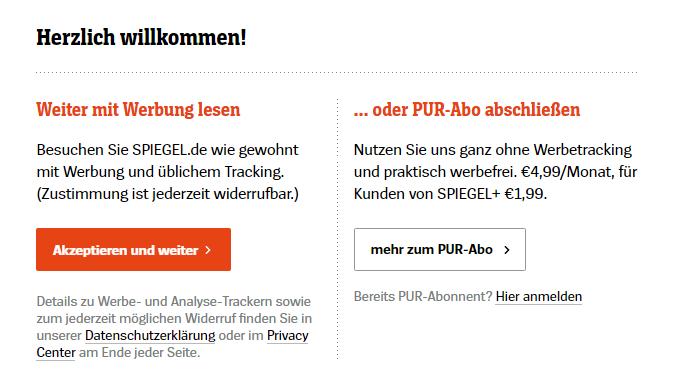
\includegraphics[width=\linewidth]{spiegel_abo_for_no_tracking}
  \caption{Eigene Aufnahme des spiegel.de Consent-Pop-ups~\autocite{Spiegel2021}}
  \label{fig:Spiegel2021}
\end{figure}

Facebook hat sich einen Besonderen Namen in dieser Dark Pattern Kategorie geschaffen, durch ihren Gründer und CEO Mark Zuckerberg in from des Dark Pattern \textit{Privacy Zuckering} von \citeauthor{Brignull} \autocite{Brignull}. Es geht dabei darum mehr Information über sich zu teilen als man beabsichtigt hat. \autoref{Spiegel2021} ist ein beispiel für ein Privacy Zuckering Dark Pattern, in dem Consent-Pop-up von spiegel.de, hat der Nutzer keine Möglichkeit die Webseite kostenlos ohne Tracking durch dirtte, wie es in der Abbildung als \enquote{üblichem Tracking} bezeichnet wird. Der Nutzer muss also Tracking und Werbung Akzeptieren oder ein Abonnement abschließen. 

% linked in beispiel aus grundlagen als teil des Gray "Social Pyramid" Dark Patterns in der unterkategorie friend spam 

\section{Schutz vor Dark Patterns}
In der Fußgängerzone stellen Hütchenspieler ihrem Publikum hohe Gewinnchancen in Aussicht, naive Passanten verstehen es als Geschicklichkeit spiel, dessen Ausgang sie durch ihr Können bestimmen, jedoch ist das ein Irrtum. Der Hütchenspieler nutzt einfache Taschenspielertricks und kontrolliert jederzeit den Ausgang des Spiels. Das Webumfeld bietet deutlich mehr Werkzeuge, um Nutzer in die irrezuführen, sodass es nahezu unmöglich ist, für einen Nutzer sämtliche Dark Patterns zu erkennen \autocite{M.Bhoot2020}. Dazu kommt das Nutzer nicht jedes Wort auf einer Webseite lesen sie überfliegen und machen Annahmen \autocite{Brignull}. Firmen können das ausnutzen, indem sie die Seite anders aussehen lassen, als was sie tatsächlich aussagt \autocite{Brignull}.

Um Nutzer zu schützen, gibt es zwei Möglichkeiten. Entweder wird der Einsatz von Dark Patterns durch den Staat reguliert oder Nutzer erkennen Dark Patterns und vermeiden Unternehmen, die diese einsetzen und regulieren den Einsatz von Dark Patterns auf diese Weise \autocite{Narayanan2020}.

Das Erkennen von Dark Patterns ist ebenso wichtig für Designer wie für Nutzer. Sie Entscheiden, ob Dark Patterns in einer Webseite vorhanden sind. Es kann sein, dass Designer A/B-Testing einsetzen und dadurch ohne es zu wissen, Dark Patterns in ein Design einzufügen \autocite{Narayanan2020}.

% Folgende Abschnitte geben Beispiele für bereits bestehende Gesetze und bewerten ihre Effektivität darin Nutzer vor Dark Patterns zu schützen. Weiterhin 

% tentative
% Wie schon der Griechische Dramatiker Euripedes sagte, \enquote{wo Gesetze schriftlich aufgezeichnet sind, genießte der Schwache mit dem Reichen gleiches Recht}. Das Bedeutet in Bezug auf Dark Patterns


\subsection{Gesetzliche Einschränkungen}
Gesetzliche Einschränkungen sind wichtig, ohne sie können Unternehmen Dark Patterns uneingeschränkt einsetzen und so Nutzer ausnutzen. Grade Dark Patterns der Kategorien Nagging und Obstruction werden selten von Nutzern erkannt \autocites{Gray_2018}{M.Bhoot2020}, deshalb können sie von Unternehmen eingesetzt werden, ohne ihre Nutzer dabei zu verärgern.

In diesem Paper wurde definiert, was Dark Patterns sind und wie sie zu erkennen sind. Nun stellt sich die Frage, wie Dark Patterns im Gesetz definiert sind. Der amerikanische Bundesstaat Kalifornien hat in seinem im November 2020 Verabschiedetem Gesetz unter Cal. Civ. Code § 1798.140(l) (Teil des \ac{CCPA}) Dark Patterns als Benutzeroberflächen, die designet oder manipuliert wurden, mit dem Effekt, das die eigenständige Entscheidungsfindung oder Wahl des Nutzers wesentlichem Untergraben oder beeinträchtigt wird.

Das ist eine sehr weit gefasste Definition, die Raum für Interpretation lässt und es den regulierenden Institutionen schwer macht, gegen rechtliche Verstöße durchzugreifen. Diese Annahme hat sich schon in Bezug auf andere Gesetze für wahr erwiesen.
Die im Mai 2018 in Kraft getretene europäische Verordnung (EU) 2016/679 (\ac{DSGVO}) die unter anderem Webseiten auffordert, Besucher ihrer Seite um Erlaubnis zu fragen, bevor sie personenbezogene Daten als Cookies speichert, sorgt zwar dafür, das fast jede Webseite den Nutzer nach seiner Erlaubnis fragt, personenbezogene Daten zu sammeln zu dürfen. Aber wie eine Studie von \citeauthor{Nouwens2020} \autocite{Nouwens2020}, die Drittanbieter Software zu Handhabung der \ac{DSGVO} Regularien mit \acp{CMP} in 680 Britischen Webseiten untersuchte, zeigt, halten sich nur 11,8\% dieser \acp{CMP} an die minimalen Standards der \ac{DSGVO}. Zudem ergab die Studie, das Webseiten Dark Patterns einsetzen, um öfter die Einwilligung ihrer Nutzer zu bekommen. Bei Seiten, die den Opt-out-Button von der ersten Seite des Einwilligungsprozesses entfernen, steigt die Anzahl der Nutzer die Einwilligen um 22–23 Prozentpunkte. Das ist ein Obstruction (\autoref{chap:Obstruction}) Dark Pattern, das zeigt wie geltende Gesetze Dark Pattern Bildung unterstützt. Eine Studie von \citeauthor{Soe2020} \autocite{Soe2020} untersuchte ebenfalls die Auswirkung der \ac{DSGVO} in 300 manuell ausgewählten Cookie Pop-ups in Nachrichtenagenturen und fanden dabei in 296 von ihnen Dark Patterns.

Ein weiteres Beispiel in der Regulierung zur Verbreitung von Dark Patterns beigetreten hat, ist das deutsche Gesetz BGBl. I S. 3352 (\ac{NetzDG}) auch Facebook-Gesetzt genannt, welches im Oktober 2017 in Kraft getreten ist. Es schreibt unter anderem vor, dass große Soziale-Netzwerke eine Möglichkeit bieten müssen, um gesetzwidrige Inhalte melden zu können. Das Bearbeiten von solchen Meldungen kostet Geld, deswegen nutzen Sozialen-Netzwerke Dark Patterns, um es Nutzern möglichst schwer zu gestalten, gesetzwidrige Inhalte zu Melden \autocite{Rieger2020}.

% https://airtable.com/shr4ACWNp9VTzuQE4/tblXgQTTipdsp7V8L
% -> 146 (https://www.ftc.gov/system/files/documents/cases/151009bunzaicmpt.pdf)

Bei der Auslegung von Gesetzen müssen in Zukunft Interface Design Entscheidungen, welche das Gesetz umgehen können oder seine Auswirkungen auf die betroffenen Unternehmen mindert, genauer in Betrachtung gezogen werden. Zudem sollte bei aktuell geltendem Recht wie der \ac{DSGVO}, die bisher kaum Konsequenzen nach sich zog \autocite{Nouwens2020}, um so Präzedenzfälle für bösartiges Interface Design wie Dark Patterns zu schaffen \autocite{Rieger2020}.

\subsection{Designer-Aufklärung}
% gives designers a bad name
% Entwickler entwickeln oft Dark Patterns ohne dass ihnen das bewusst ist
Der Zweck von Design ist es Nutzer zu überzeugen etwas zu tun, das bringt potenzial den Nutzer auszunutzen \autocites{OinasKukkonen2009}{Sengers2005}. Designer sollten besorgt über die Verbreitung von Dark Patterns sein, sie gelten als unethisch und wirken sich lecht auf ihre Reputation aus \autocite{Narayanan2020}.

Design können für ein bestimmtes Publikum gutartige Endscheidungen treffen, welche aber für ein breiteres Publikum in manipulatives Design müden kann \autocite{Gray_2018}. Endscheidungen die für ein breites Publikum geschaffen werden können Dark Patterns produzieren, das ist bei A/B-Tesing der fall. A/B-Testing wird häufig in der Webentwicklung eingesetzt, da so Annahmen mit Daten untermauert werden können \autocite{Kohavi2017}. Für A/B-Testing werden häufig Daten genommen, die wichtig für die Bilanz des Unternehmens sind \autocites{Kohavi2017}{Narayanan2020}. Das führt dazu, dass Designer unbewusst und ohne eine böse Absicht Dark Patterns in die Webseite einbinden \autocite{Narayanan2020}.

Moralisch deutlich bedenklicher sind die Fälle in denen Designer Dark Patterns bewusst einsetzen, aus eigenem willen oder durch Druck von vorgesetzen. Dabei müssen designer nicht über Dark Patterns, sondern über ihre folgen bei Nutzern aufgeklärt werden, um entweder an Ihre Moral zu appelieren oder darauf, dass sie einen Negativen effekt auf Nutzerbindung und somit auf Profit haben kann. Ein weiterer vorschlag von \citeauthor{Gray_2018} \autocite{Gray_2018} ist, dass sich Designer Ethischen Verordnungen verpflichen wie es beispielsweise bei Ärtzen der Fall ist. 

\subsection{Nutzer-Aufklärung}
% subreddit '/r/assholedesign' \autocite{Chivukula_2019}
% Brignull klärt auf seiner Seite auf \autocite{Brignull}
% Nutzer aufklären, führt zur Reduzierung des Erfolges von Dark Patterns, was wiederum dafür sorgt, dass Dark Patterns sich für Firmen weniger lohnen und sie auf diese verzichten
Laut \citeauthor{Brignull} \autocite{Brignull} ist der beste Schutz vor Dark Patterns, sie sich bewusst zu machen und die Firmen, die sie benutzen, zu boykottieren. \autoref{chap:Psychologie} zeigt, dass der Mensch anfällig für Dark Patterns sein kann. 41.4\% der Befragten einer Studie von \citeauthor{M.Bhoot2020} \autocite{M.Bhoot2020} gaben an, noch nie von einer Webseite ausgetrickst worden zu sein, jedoch hat keiner der Befragten alle zwölf Dark Pattern die Gegenstand der Studie waren, identifizieren können. Dabei wurde Auftrittshäufigkeit als wichtigsten Gesichtspunkt zur Identifikation von Dark Pattern erkannt. Deshalb ist es wichtig, Nutzer über Dark Patterns aufzuklären, sodass sie diese leichter erkennen, um sich selbst vor ungewollten Konsequenzen schützen können.

In den letzen Jarhen gewann der Dark Pattern Begriff immer mehr an bedeutung \autocite{Chivukula_2019}, er wurde zum Schlagwort in Massenmedien und der Politik, repräsentativ für manipulatives Interface Design. Je mehr über Dark Patterns gesprochen wird, desto bewusster werden sie den Nutzern und je mehr Nutzer Dark Patterns erkennen und aus dem Weg gehen, desto weniger effektiv sind sie für Unternehmen. Sobald Dark Patterns nicht rentieren für Unternehmen gibt es keinen Anreiz sie einzusetzen.

\section{Fazit und Ausblick}
% wie erkennt man Dark Patterns?
% • Signals of scarcity and urgency: they push us to act quickly
% • Default selections: we stick to the choices that are made for us
% • Emphasize on the benefits of accepting (manipulation)
% • Obligation to accept to use a service
% -> benifts the provider not the user

% wiederholung für desiner wiederholen

% webseiten könnten sich als alleinstellungs merkmal ein zertifikal als darkpattern frei geben lassen (gibt keinen der das macht, würde geld kosten und wer überprüft das)

% grade die nur schwer erkannten dark patterns sind das problem, da die nutzer nicht mitbekommen das sie ausgenutzt werden und somit muss der betreiber auch kaum konsequenzen fürchten und fühlt sich bestärkt in seinem einsatz des Dark Patterns
% --- oben und unterndrunter kombinieren? --- 
% es gibt drei gruppen von Nutzern, die erste die ihre ausnutzung nicht wahr nimmt, die zweite die es nicht interessiert und die dritte die es sich nicht gefallen lässt und konsequenz beispielsweise die webseite nicht mehr nutzt. Solange die ersten beiden gruppen groß genug sind um bei dem Anbieter der Website für einen gewinn zu sorgen werden sie Dark Patterns einsetzen.

% sometimes the only way to protect yourself from a dark pattern is to stop using the service, but in case of some servicses there are not good alternative for example in case of facebook there are no alternative socal networks where you have the same connection as in facebook so u cant switch off it

% Abkürzungsverzeichnis
\begin{acronym}[IEEE]
  \acro{CCPA}{California Consumer Privacy Act}
  \acro{DSGVO}{Datenschutz-Grundverordnung}
  \acro{NetzDG}{Netzwerkdurchsetzungsgesetz}
  \acro{CMP}{Consent Management Platform}
\end{acronym}

% Literaturverzeichnis
\addcontentsline{toc}{section}{Literatur}
\printbibliography
\end{document}
// bill zitieren mit namen